% !TEX root = C:\Users\Jan\Documents\dev\Risk-Measurement-Framework\masterthesis_tex\masterthesis_main.tex

\section{Risk Measurement Framework concept and design}
\label{sec:conFrame}

In contrast to Schwerdtner et al. \cite{DBLP:journals/corr/abs-2011-04328}, the framework of this thesis concentrates on training, especially risk measurement before and during training of the ML model. This section discusses and explains the design of the RMF. The RMF is a technical framework based on a concept to measure risks of backdoor attacks \cite{DBLP:conf/eusipco/ArshadAQLY21} by measuring the attacker's effort and extent of damage of an attack. \\ Referencing on this thesis approach from Biggio et al. \cite{DBLP:conf/icml/BiggioNL12} a security analysis for ML is that the attacker knows the ML model and can use the data from the data distribution platform. It is assumed for the RMF that the attacker knows the training data. This is an unrealistic assumption, but in real-world scenarios the attacker could use a surrogate training set instead, from the same data distribution platform which the developers use \cite{DBLP:journals/ml/BarrenoNJT10}. The following subsection goes to the research question \ref{itm:rq1} - How can the procedure and requirements from ISO 27004 be used for risk measurement of ML models?

\subsection{Using the standards for the risk measurement}
\label{sec:standard}

After the explained measures and measurement development based on ISO 27004 in section \ref{sec:relWork}, the next step is to map requirements into the RMF. This discussion what parts of them can be fulfilled and which parts can not fulfilled before using the RMF. \\ \\

\textbf{''Defining the measurement scope''} is the first requirement about the organization's capabilites and resources which define the initial scope. It starts by decisions of the management and can not be fulfilled by the RMF because that is an individual process specific for an organization and stands not in relation with the risk measurement in the RMF. The part defining stakeholder can not be fulfilled but in ''Developing measurement constructs'' it will be further discussed how to identify them.  \\ \\

\textbf{''Identifying an information need''} is as the name says about the identification of an information need. The first activity of identifying the processes and examination of the ISMS can not be fulfilled because the RMF stand in no relation with an ISMS directly. The information need prioritization criteria such as risk treatment can be fulfilled by the general riks measurement because all results are shown as transparent as possible. The organization's capabilities and resources criteria is individual for the organization and can not be measured. The interest of stakeholders are individual and must be defined before using the RMF. The third activity can be fulfilled by showing all results of the risk measurement which appendix \ref{sec:template} shows. The last acitivity is a process about documenting and communicating with the stakeholder which can be fulfilled after using the RMF because every risk measurement step is documented. \\ \\

\textbf{''Selecting the object of measurement and its attributes''} describe that objects and attributes are identified in the scope and context of an ISMS. The identified objects and attributes are related to the risk indicators which are used to measure risks and calculate the final risk. As Figure \ref{fig:relation_risk_ind} shows, the risk indicators are represented by objects and attributes in the ISO 27004 \cite{ISO_27004_2009} standard. In order to assign the terms of objects, attributes, and base measures to the RMF, all risk indicators are assigned to these standard terms. When this allocation takes places, this is always mentioned.

\begin{figure}[ht!]
  \centering
  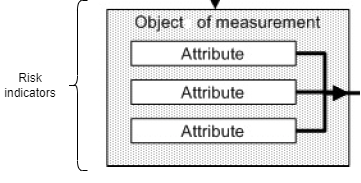
\includegraphics[width=10cm]{pictures/relation_risk_ind.png}
  \caption{Relation between the objects, attributes and the risk indicators adapted from \cite{ISO_27004_2009}.}
  \label{fig:relation_risk_ind}
\end{figure}

The terms of the standard thus enable a better classification and relationship of the terms assigned to the risk indicators. In order of this requirement, attributes identify the type of measurement methods to obtain values which are assigned to the base measures. To fulfill the relation between the measurement methods that are selected through the attributes, there is a need to relate the attributes with a measurement method. For more detailed explanations of the measurement methods the following subsections go into the individual points of the concept for the RMF. \\ \\

\textbf{''Developing measurement constructs''} is about to define a measure selection, measurement method, measurement function, the analytical model, indicators, decision criteria, and stakeholders. Starting by identify a measure selection the following example criteria from ISO 27004 should help: facilitation for data collection, facilitation for interpretation, measures to calculate costs of analysing, and collecting the data. The data collection can be done through the measurement methods. All of the collected data should be used for interpretation, for the attack, and the attacker's effort. Specificlly on poisoning attacks the training data must be analyzed and any information can be used for the measurement process. It is complicated to find poisoned data because the modifications are small in images which can be harder to get these information. The success depends on the patch size and the attacks on an image are highly specified \cite{DBLP:conf/icml/SchwarzschildGG21}. Therefore it is clearer to define the risk indicators as the measure selection because it measures certain values that are common for a particular attack. \\ The measurement method is used to quantify the measurement object by transforming the attributes into the value that is assigned to the base measure. Measurement methods can be subjective or objective. The objective measurement methods measure based on the data that are given from an attack. The subjective measurement methods are based on human judgment as, for example, with the threat model of Doynikova et al. \cite{DBLP:conf/crisis/DoynikovaNGK20}.

\begin{figure}[ht!]
  \centering
  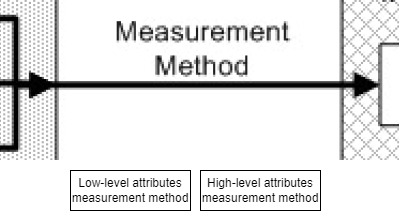
\includegraphics[width=10cm]{pictures/measurement_methods.png}
  \caption{The measurement method (right) send the collected data to the measurement method left (left). Both measurement method are executed at the second step of the measurement from ISO 27004 -  adapted from \cite{ISO_27004_2009}.}
  \label{fig:measurement_methods}
\end{figure}

The outputs of the measurement methods need to be assigned to the base measures. Every base measure is an attribute from the objects but with
an assigned value in the RMF. These base measures are used as the input for the measurement functions which are calculations to transform them into derived measures or can be directly handed over to the analytical model. The measurement functions are calculations to transform the base measures into derived measured. In context to the risk measurement of the RMF this can be fulfilled for values which are not calculated already for example, the accuracy is a risk indicator that is already a total value \cite{9783960101925} and do not need a further calculation with other results from the measurement method's output. \\
After explaining the derived measure the next step in the measurement is the analytical model. For each indicator there should a analytical model by transforming values that are defined to a base or derived measure. Indicators are assigend values to aggregated values which in turn are assigned to derived measures and/or base measures. The analytical model creates outputs that are relevant for all stakeholders. However, this connection to the stakeholders is not considered further in this thesis. The values that are assigned to indicators and how they are presented describe ''Establishing data collection and analysis processes and tools''. \\
If the indicators are evaluated the decision criteria are the penultimate step before the measurement results. Decision criteria are based on historical data, plans, and heuristics or calculated as statistical control or confidential limits. That process can not be fulfilled because the basis of the decision criteria is a part which should be present before executing the RMF on a ML model. \\
The last requirement is defining stakeholders. Stakeholders can be clients, reviewers for measurement, information owners or information communicators \cite{ISO_27004_2009} which can be identified as Sharp et al. \cite{DBLP:conf/dexaw/SharpFG99} explain in their work.

\begin{figure}[ht!]
  \centering
  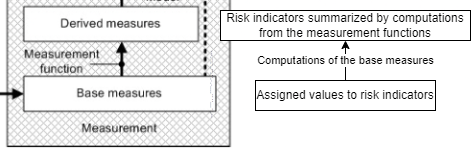
\includegraphics[width=10cm]{pictures/base_to_derived_measure.png}
  \caption{After the measurement methods are finished, the outputs are assigned to base measures and named as the risk indicators. A few risk indicators are calculated to derived measures - adapted from \cite{ISO_27004_2009}.}
  \label{fig:base_to_derived_measure}
\end{figure}

Figure \ref{fig:base_to_derived_measure} shows the process (of this requirement) after the measurment methods are finished and assigned their output to the base measures.\\ \\

\textbf{''Applying measurement constructs''} is the requirement that explains which information the measurement construct should contain. These information are the purpose of measurement, measurement objects, collected and used data, the data collection process and analysis, the process that reports measurement results, stakeholders and their roles and responsibilities, and a cycle to ensure the usefulness of measurements including the relation to the information needs \cite{ISO_27004_2009}. In context to the RMF the stakeholders and their roles and responsibilities, and the cycle to ensure the usefulness of measurements including the relation to the information needs can not be fulfilled. These information are not gathered from the RMF and it is not the goal of the RMF to collect these information. \\ \\

\textbf{''Establishing data collection and analysis processes and tools''} is the process of collecting and analysing data to identify how the data is collected and stored with its necessary information in the developed measurement results based on two activities. This process can be fulfilled in all individual processes of the risk measurement in the RMF. The first acitivity is how to store the collected data. The neccessary information are date, time, location of the data collection, information collector, information owner, any issues that happened during data collection, information for verification and measurement validation, and verify data against measure selection criteria and measurement constructs validation criteria. \\ The second acitivity can not be fulfilled by the RMF because it requires a communicator and stakeholders which analyse and interpret the data by human judgment. \\ \\

\textbf{''Establishing measurement implementation approach and documentation''} is the last requirement and describe the needed information from an implementation plan. This plan is not the basis of the RMF because the process depends on organization's specifications and plans as a calendar which this thesis not using to design and implement the RMF. Instead of this implementation plan, subsection \ref{sec:final_design} show the final structure after which the RMF is implemented. \\ \\

In conclusion, with regard to the research question \ref{itm:rq1}, it can be stated that the requirements mentioned reflect only recommendations. That makes it possible to fulfill the requirements for security improvements in ML and confirms the hypothesis \ref{itm:h3} regarding to the requirements and procedures of ISO 27004.

\subsection{Risk indicators}
\label{sec:risk_indicators}

The selection of the risk indicators is the first part of the RMF to fulfill the requirements. Risk indicators are in context of ISO 27004 \cite{ISO_27004_2009} attributes and represent the input data. The input data are an object's attributes and assigned to the corresponding measurement method. Breier et al. \cite{DBLP:journals/corr/abs-2012-04884} in subsection \ref{sec:approaches} present proposals that are the approach for the proposals of the risk indicators. These proposals are attack specificity, attack time, attacker's knowledge, and attacker's goal. The proposals have different subcategories which are visualized in figure \ref{fig:classifi_attacks_ml}.

\subsubsection*{Attributes and objects based on ISO 27004}

For the RMF the objects are the attack and the attacker. To measure the risks on backdoor attacks, the first step is the selection of objects and associated attributes. \\ Beside of the proposed risk indicators defined by Breier et al. this thesis use further risk indicators such as the accuracy of a ML model \cite{DBLP:journals/soco/GarciaFLH09}, the computational resources, and the TP, FP, TN, FP \cite{DBLP:journals/symmetry/PhamJAADYPNLGPT20}. Through their assignments to the two objects they are in turn assigned to the measurement methods which Figure \ref{fig:measure_damage} and \ref{fig:measure_effort} show. These risk indicators are set out in hypotheses \ref{itm:h1} and \ref{itm:h2}.

\begin{figure}[ht!]
  \centering
  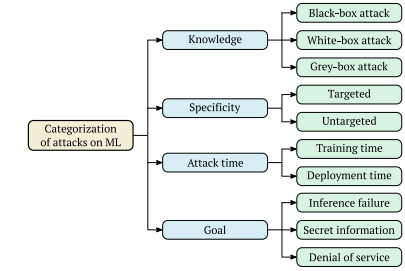
\includegraphics[width=10cm]{pictures/classifi_attacks_ml.png}
  \caption{Attack classifications on ML adapted from \cite{DBLP:journals/corr/abs-2012-04884}. The grey-box attack is not observed in this thesis.}
  \label{fig:classifi_attacks_ml}
\end{figure}

\subsection{Measurement methods}

Risk measurement starts after the identification of suitable objects and attributes \ref{sec:risk_indicators} with the selection of measurement methods according to the requirements and procedure of ISO 27004. The measurement methods start by using backdoor attacks. As already mentioned in the related work section \ref{sec:relWork}, there are different possibilities to execute poisoning attacks. At first, it is important to train a ML model without an attack to get the original values.
Xiao et al. \cite{DBLP:conf/sp/XiaoLZX18} describe that training data can be polluted or mislabled when they come from external sources. This means that it is important where the training data comes from to determine, for example, how trustworthy these data are. Furthermore, Turner et al. \cite{turner2018clean} train a classifier with a
small set of clean input data where the input data are images from a trusted source that obtained or inspected the data. So, the more trustworthy a set of training data is, the lower the risk will be. For this thesis this process is skipped and the RMF can not check where the trainign data come from. The measurement methods expect only what should be measure by the attributes and which attack should be executed on the ML model. A ML model can be outsourced (Machine Learning as a Service, or MLaaS \cite{DBLP:journals/corr/abs-1708-06733}), self-developed, come from an external resource and only has to be trained. For example, Google's Cloud Machine Learning Engine \cite{google_ai2022} allow's users to upload training data and a TensorFlow ML model to train it in the cloud \cite{DBLP:journals/corr/abs-1708-06733}. Also at this point, no decision is made between these possibilities. Instead of the distinctions, everything is executed locally. This in turn allows to assign all risk indicators at each part in the ML model. \\ The first measurement method should measure the values to evaluate the extent of damage. The other measurement method is used to find the attacker's effort. Both work according to the threat model of Doynikova et al. \cite{DBLP:conf/crisis/DoynikovaNGK20} by analyzing the data before and after an attack. Therefore the measurement method to measure the extent of
damage must be executed before measuring the attacker's effort. The following sections \ref{sec:charac_backdoor}, \ref{sec:backdoor_types}, \ref{sec:ext_dmg}, \ref{sec:find_effort}, and
\ref{sec:use_threat_model} explain the concept of the measurement methods in the RMF.

\subsection{Characteristics of backdoor attacks}
\label{sec:charac_backdoor}

After discussing and evaluating the standards for the risk measurement in the RMF in section \ref{sec:standard}, this subsection explains which characteristics of backdoor attacks are measured in the
RMF. Biggio et al. \cite{DBLP:conf/icml/BiggioNL12} explain that poisoning attacks and therefore also backdoor attacks are causative attacks which means manipulations against training data is the focus of them. Further, Xiao et al. \cite{DBLP:conf/sp/XiaoLZX18} describe that training data can be polluted or mislabled when they come from external sources. Xiao et al. explain that poisoning attacks are not based on software vulnerabilities, which means that software bugs are not the execution point of backdoor attacks when implementing them into the RMF. This means the RMF measures conspicuities in the training data and measures the computational resources. Furthermore, the RMF measures before and after an attack to compare the differences between the original and manipulated ML model.

\subsection{Types of backdoor attacks}
\label{sec:backdoor_types}

The following backdoor attacks should be used to represent possible attacks on a ML model. Further, this subsection should show the main principles of the backdoor attacks that are used in the RMF.

\subsubsection*{Backdoor attack concepts}

\textit{Pattern Backdoor Attack}, \textit{Clean Label Backdoor Attack}, and \textit{Hidden Trigger Backdoor Attack} are the three backdoor attacks for this thesis. \\ \\
\textbf{Pattern Backdoor Attack} Gu et al. \cite{DBLP:journals/corr/abs-1708-06733} explain \textit{Pattern Backdoor Attack} which goal is to change original labels to a target label on outsourced ML models. This happens by attacking a random small selection of the training set and apply a backdoor trigger into the input data. To be more precise, a backdoor attack works by adding a trigger in form of a pattern into some images in the training set, depending on the attack specificity (targeted or untargeted). Targeted means to poison specific images of a label that should trigger the backdoor if a pattern is on the images. Untargeted is an attack specificity through which images are random from a random label. \\ After a successful attack it is difficult to detect backdoor attacks because the ML model's performance does not change noticeably in relation to the original performance \cite{DBLP:journals/corr/abs-2106-07925}. Further, backdoor attacks are powerful, because they take control over images that should be misclassified while the ML model is in test time \cite{turner2018clean}. In their work, Gu et al. show different backdoor attacks and perform a case study with a traffic sign detection attack on a neural network. The evaluated backdoors are a single pixel backdoor and a pattern backdoor. The single pixel backdoor increases the brightness of a pixel and the pattern backdoor adds a pattern of bright pixels in an image which Figure \ref{fig:backdoor_pattern} shows.

\begin{figure}[ht!]
  \centering
  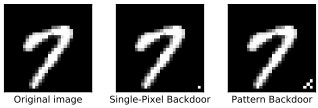
\includegraphics[width=10cm]{pictures/backdoor_pattern_bad_net.jpg}
  \caption{Backdoors in relation to the original image adapted from \cite{DBLP:journals/corr/abs-1708-06733}.}
  \label{fig:backdoor_pattern}
\end{figure}

The implemented attacks from Gu et al. are a Single Target attack and an All-to-All attack where the training data is poisoned \cite{DBLP:conf/ccs/HuangJNRT11}. Single Target attacks use the single pixel backdoor by mapping a label from a digit (that is an image of the MNIST \cite{LeCun1995LearningAF} training set) $i$ as a digit $j$ on backdoored inputs. Figure \ref{fig:mapped_from_i_to_j} represents the classification error of the color-coded values where the row is $i$ and the column $j$.

\begin{figure}[ht!]
  \centering
  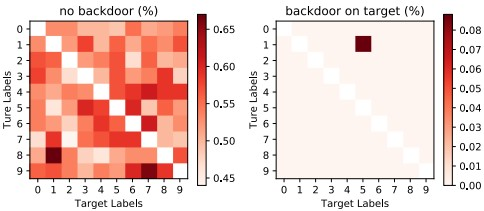
\includegraphics[width=10cm]{pictures/mapping_from_i_to_j.jpg}
  \caption{The left side shows the classification error (\%) of clean images with a Single Target attack for every instance. The right side shows the same but with backdoored images - adapted from \cite{DBLP:journals/corr/abs-1708-06733}.}
  \label{fig:mapped_from_i_to_j}
\end{figure}

The attack strategy is a random pick of images from the training data and implements a poisoned version back to the training set. An All-to-All attack changes a digit label $i$ to $i + 1$. After testing the All-to-All attack, the original ML model has an error rate of 0.03\% while the ML model with the backdoored image has an average error of 0.56\%. \\ The case study is a traffic sign detection attack where the label of a stop sign is changed to a label of a speed limit sign. The backdoor of the image is either a yellow square, bomb image, or a sunflower image as the size of a post-it note on the stop sign. These backdoors are found at the bottom of the stop sign.

\begin{figure}[ht!]
  \centering
  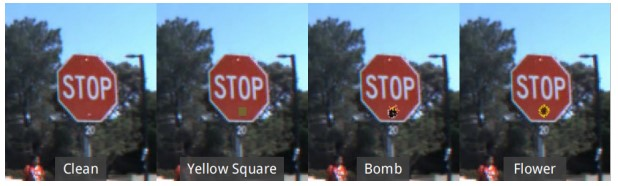
\includegraphics[width=10cm]{pictures/stop_sign.jpg}
  \caption{Stop sign as the clean version and with the three backdoors adapted from \cite{DBLP:journals/corr/abs-1708-06733}.}
  \label{fig:stop_sign}
\end{figure}

The setup for the case study of Gu et al. bases on the Faster-RCNN \cite{DBLP:conf/nips/RenHGS15}. The Faster-RCNN takes an image as input data and the output data is a proposal as a set of rectangular objects where every rectangle has an objectness score.

\begin{figure}[ht!]
  \centering
  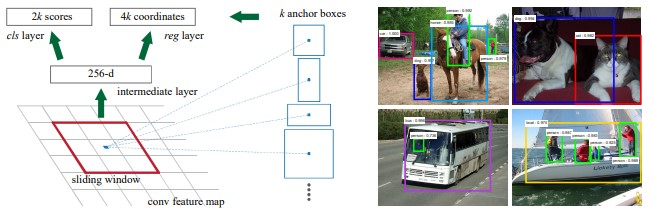
\includegraphics[width=10cm]{pictures/f_rcnn.jpg}
  \caption{The left side shows a region proposal network which represents the Faster-RCNN network and the right side shows an example of the detection adapted from \cite{DBLP:conf/nips/RenHGS15}.}
  \label{fig:f_rcnn}
\end{figure}

The attack is a Single Target attack where the label of the stop sign image changes to a speed-limit label, and a random target attack where the stop sign is randomly changed to an incorrect label. The results show a successful pass of the validation tests and 90\% of the stop signs are missclassified as speed-limit signs. Gu et al. tested their ML model in a real-world attack by pasting a sticker on a stop sign near their office building. The ML model classified the stop sign with a 95\% confidence as a speed-limit sign. The ML model's accuracy is decreased on backdoors to 1.3\% which makes a misclassification to more than 98\%. This attack is now transferred to the RMF for risk measurement to check how much the accuracy is reduced. The more the accuracy for the classification of the poisoned images is decreased, the higher is the possible extent of damage which increases the risk. \\ \\

\textbf{Clean Label Backdoor Attack} In their work, Turner et al. \cite{turner2018clean} explain \textit{Clean Label Backdoor Attack} attacks in direct comparison to Gu et al. \textit{Pattern Backdoor Attack}. Turner et al. show an approach for executing backdoor attacks by utilizing adversarial examples and Generative Adversarial Network (GAN)-generated data. The approach of Turner et al. is analyzing the effectiveness of the attack of Gu et al. while a simple technique is applied for data filtering. Data filtering is a technique to find poisoned data by comparing the used training data with trusted training data. Turner et al. discovered that the poisoned inputs are outliers and are clearly wrong from the human inspection side. The attack would be ineffective if it would rely solely on poisoned inputs which are labeled correctly and evade such filtering. At this point Turner et al. created an approach that poisons inputs which appear plausible to humans. The inputs need small changes to make them harder while classifying them but the original label must still remain plausible. This transformation is performed by a GAN-based interpolation and adversarial bounded pertubations. GAN-based interpolation takes each input into the GAN latent space \cite{DBLP:conf/nips/GoodfellowPMXWOCB14} and then interpolate poisoned samples to an incorrect class. Adversarial bounded pertubations use an optimization method to maximize the loss of the pre-trained ML model on poisoned inputs while staying around the original input. The main focus of this attack are poisoned samples that still have poisoned labels. That is why the attack is called Clean Label attack which is originally from \cite{DBLP:journals/corr/abs-1804-00792} in context of targeted poisoning attacks. Figure \ref{fig:poisoned_clean_label} shows an example airplane with different poisoned samples. The experiments base on the same patterns with a small black-and-white square in the bottom-right corner of the poisoned images as Gu et al. use in their work. The classifier is trained with the poisoned data and the test data are not labeled. The training dataset for the experiments
is the CIFAR-10 dataset \cite{Krizhevsky2009LearningML}. The ML model is a trained Wasserstein GAN \cite{DBLP:journals/corr/ArjovskyCB17}, \cite{DBLP:conf/nips/GulrajaniAADC17}. A GAN is strategy for training data where a game is defined between two competing networks. It contains a generator network and maps a noise source into the input space. A second network is the discriminator network which receives a generated sample or true data sample and then it must distinguish between those two samples. The Wasserstein GAN is using the Earth-Mover distance which is also called Wasserstein-1. For
further explanation of the mathematical structure, please see \cite{DBLP:journals/corr/GulrajaniAADC17}.

\begin{figure}[ht!]
  \centering
  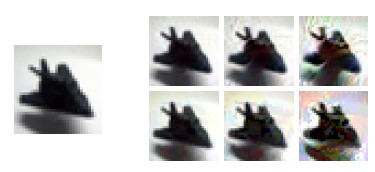
\includegraphics[width=10cm]{pictures/poisoned_clean_label.jpg}
  \caption{Difference between an original image and the conversion into adversarial examples with different pertubations adapted from \cite{turner2018clean}.}
  \label{fig:poisoned_clean_label}
\end{figure}

\textbf{Hidden Trigger Backdoor Attack} The last backdoor attack from Saha et al. \cite{DBLP:journals/corr/abs-1910-00033} is the \textit{Hidden Trigger Backdoor Attack} which goal is to let poisoned data look natural with correct labels. This backdoor attack uses a threat model defined from Gu et al. \cite{DBLP:journals/corr/abs-1708-06733}. In this threat model, the attacker provides poisoned training data to a victim that uses it with a pre-trained ML model. The attacker uses a small image as a backdoor which changes the target label to a specific wrong label. This can be used for both attack specificity, targeted and untargeted. With this threat model it is possible to identify the poisoned data because as already explained in \textit{Clean Label Backdoor Attack}, the missclassified images change their label. Identifying the poisoned data in a training set can show how many images are poisoned to measure the extent of possible damage. Saha et al. propose a threat model inspired
from Shafahi et al. \cite{DBLP:journals/corr/abs-1804-00792} and Sabour et al. \cite{DBLP:journals/corr/SabourCFF15} where the poisoned data are labeled correctly and the backdoor also remains not visible. This is done through optimization for poisoned images which pixel space is close to images from a target category while its feature space is close to source images that are patched with the backdoor. The next part is generalizing the attack for unseen source images which means that the trigger cannot be found during poisoning. Also the trigger should be placed at any random location. In order to implement this, during the optimization the poisoned images pushed close to a cluster of source images that are patched. Based on the
work of Moosavi-Dezfooli et al. \cite{DBLP:conf/cvpr/Moosavi-Dezfooli17} about universal adversarial examples, Saha et al. minimized the value of loss at all source images and trigger locations. This is done by choosing a random trigger location and source images for each iteration of optimization. Over every iteration a method optimizes randomly patched source images and assigns them to poisoned images closest to the feature space.

\begin{figure}[ht!]
  \centering
  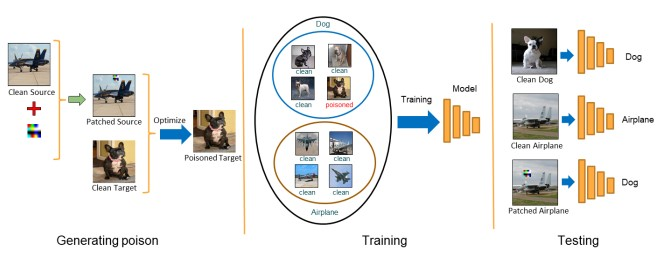
\includegraphics[width=10cm]{pictures/procedure_hidden_trigger.jpg}
  \caption{The left side visualize how an attacker generates a set of poisoned images. In the middle the visualization shows how the training data is extended by the poisoned data and then the victim trains the ML model. The right side visualize the test time. An attacker adds the backdoor trigger to images with the source category to manipulate the ML model without changing the label. This visualization is adapted from \cite{DBLP:journals/corr/abs-1910-00033}.}
  \label{fig:procedure_hidden_trigger}
\end{figure}

\begin{figure}[ht!]
  \centering
  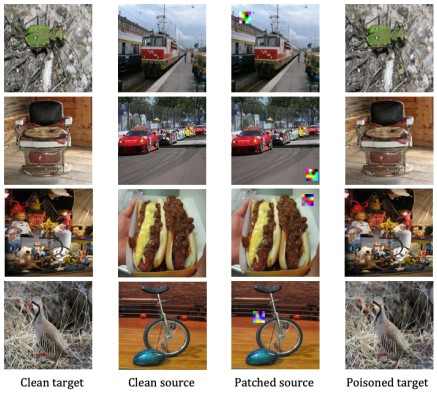
\includegraphics[width=11cm]{pictures/poisoned_hidden_trigger.jpg}
  \caption{The left side visualize how an attacker generates a set of poisoned images. In the middle the visualization shows how the training data is extended by the poisoned data and then the victim trains the ML model. The right side visualize the test time. An attacker adds the backdoor trigger to images with the source category to manipulate the ML model without changing the label. This visualization is adapted from \cite{DBLP:journals/corr/abs-1910-00033}.}
  \label{fig:poisoned_hidden_trigger}
\end{figure}

\subsection{Measurement method for the extent of damage}
\label{sec:ext_dmg}

Based on the attacks, this subsection explains how the extent of damage is measured. As the hypotheses \ref{itm:h1} assumes, the attack specificity, attack time, and the TP, TN, FP, FN are risk indicators. Based on \cite{DBLP:journals/corr/abs-1708-06733}, \cite{turner2018clean}, and \cite{DBLP:journals/corr/abs-1910-00033}, the accuracy metric of a ML model for a specific image is a value that represents the success of a backdoor attack. All of these risk indicators are assigned with values before and after an attack during the training of a ML
model. These data can be collected directly from the ML model which represents the low-level attributes in the threat model from Doynikova et al. \cite{DBLP:conf/crisis/DoynikovaNGK20}. To get these assigned data the RMF needs a measurement method based on the low-level attributes. The attack time and attack specificity are both mapped to the high level attributes as Figure \ref{fig:attribute_mapping} shows. The attack time measures the time an attack needs to be executed in relation to the training without executing an attack. The time also differentiate between the training and inference time. The first time measurement is for the attacker's effort while the second part of this risk indicator checks the ML model during training or inference for possible vulnerabilites \cite{DBLP:journals/csur/RosenbergSER21} in the training or test dataset. For example, if the attacker wants to implement a backdoor attack he than have to be only concentrate on the training dataset for vulnerabilites. After the training the RMF assigns the values of the risk indicators to the base measures which is the conclusion of the measurement methods.

\begin{figure}[ht!]
  \centering
  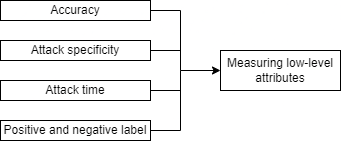
\includegraphics[width=9cm]{pictures/measure_damage.png}
  \caption{Risk indicators of the attack object in relation to the low-level attributes measurement method.}
  \label{fig:measure_damage}
\end{figure}

\subsection{Measurement method for the attacker's effort}
\label{sec:find_effort}

After explaining the procedure to get the base measures to measure the extent of damage, this subsection explains how the base measures for the attacker's effort are measured. Breier et al. \cite{DBLP:journals/corr/abs-2012-04884} propose the attacker's knowledge and goal. Further, theses proposals and the computational resources as hypotheses \ref{itm:h2} describe are used as the risk indicators. Starting with computational resources that are a need to train a ML model. This riks indicator gets the current use of the central processing unit (CPU), graphics processing unit (GPU), and memory resources to find out what an attacker needs to test and execute his attack. The attacker's knowledge is divided into two possible knowledge levels. The first knowledge level are black-box attacks where the attacker has no information about the ML model. \\
In their work, Papernot et al. \cite{DBLP:conf/ccs/PapernotMGJCS17} explain a black-box attack strategy to misclassify a deep neural network (DNN) \cite{DBLP:journals/spm/X12a} by generated adversarial examples. Papernot et al. assume that the attacker has no knowledge about the structure, parameters, and does not have access to any training set that this DNN uses. The attack strategy has no need to train an independent training dataset. The goal is to train a DNN with synthetic input data and generated from the adversary. Synthetic datasets are reflecting real datasets by preserving their relations between the variables and statistical properties \cite{Quintana2020ASD}. The output data are assigned labels from the targeted DNN and the adversary observe the output data. The input data are handwritten digits as
images and the output data are one of these digits. The aim of the attack is to get a minimal altered version of each input which is called an adversarial example. This should misclassify the input data by a minimal pertubation. This happens by generating the synthetic dataset which the adversary generates.\\
The second knowledge level are white-box attacks where an attacker has nearly perfect knowledge about the ML model. Prinz and Flexer \cite{DBLP:journals/corr/abs-2007-14714} present end-to-end adversarial attacks on classifications of music instruments. The training data are from the DCASE2019 Challenge \cite{DBLP:conf/dcase/FonsecaPFES19}. In their work, Prinz and Flexer use four adversarial white-box attacks. Two attacks are untargeted and called Fast Gradient Sign Method (FGSM) \cite{DBLP:journals/corr/GoodfellowSS14} and Projected Gradient Descent on the negative loss function (PGDn) \cite{DBLP:conf/iclr/MadryMSTV18}. The other two targeted attacks are adaptions from the Carlini and Wagner (C\&W) \cite{DBLP:conf/sp/Carlini018} method. The architecture is a convolutional neural network (CNN) \cite{DBLP:journals/corr/Kim14f} as Figure \ref{fig:cnn_whitebox} shows.

\begin{figure}[ht!]
  \centering
  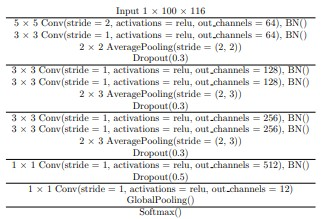
\includegraphics[width=8cm]{pictures/cnn_whitebox.jpg}
  \caption{The neworks contains $5x5$ and $3x3$ convolutional layers with the ReLU activation, batch normalisation, and average-pooling layers. The CNN uses dropout for regularisation and the final layer is a $1x1$ convolutional layer adapted from \cite{DBLP:journals/corr/abs-2007-14714}.}
  \label{fig:cnn_whitebox}
\end{figure}

PGDn is an attack on a negative loss function \cite{DBLP:journals/corr/MadryMSTV17} which goal is increasing on a sample the negative loss interatively. FGSM is a method which goal is to increase the loss by moving a scaled step in gradient direction while the adversarial pertubation is computed \cite{DBLP:journals/corr/GoodfellowSS14}. C\&W's first method is about using gradient descent to minimise the loss to a specific class. The Multi-Scale C\&W attack keeps pertubations small with the squared norm \cite{DBLP:conf/sp/Carlini018}.
Prinz and Flexer \cite{DBLP:journals/corr/abs-2007-14714} and Papernot et al. \cite{DBLP:conf/ccs/PapernotMGJCS17} show both ways to attack ML models and in both works they used specific attacks for specific ML models. Both attacks bases on white-box or black-box attacks which shows that it is possible to find out if an attack is a black- or white-box attack. And after that is found out it should be possible measure the knowledge by pre-determined steps to execute the attack \cite{bsi_2013}. To measure the attacker's knowledge for black- and white-box attacks, the explained attacks in \ref{sec:charac_backdoor} should represent these attacks. \textit{Hidden Trigger Backdoor Attack} \cite{DBLP:journals/corr/abs-1910-00033} is an attack where the attacker uses a backdoor trigger on a pre-trained ML model with finetuning for classification. The backdoor trigger must be implemented while finetuning the ML model to change the label. When the ML model finetunes its training data, the attacker changes the source label to a target label. \textit{Clean Label Backdoor Attack} \cite{turner2018clean} is an attack which misclassifys instead of inference, during training time. With this goal, the images should be harder to be correct classified and the ML model should recognize the backdoor trigger as a feature. That should prevent modificatons during training time of the poisoned data. This attack is implemented based on projected gradient descent (PGD) \cite{DBLP:journals/corr/MadryMSTV17}. PGD is an approach to train NN with a improved resistance against adversarial attacks.
\textit{Pattern Backdoor Attack} \cite{DBLP:journals/corr/abs-1708-06733} is an attack which adds a pixel pattern or single pixel into an image and misclassifies these poisoned images to a target or untargeted label. After adding the pattern these poisoned images have to be mixed back into the original training dataset. The attacker's goal is the last risk indicator to measure the attacker's effort to find out what the attacker is trying to achieve \cite{DBLP:journals/corr/abs-2012-04884}. To find this goal in the measurement method, this risk indicator has to know which attack is used. If this attack clarified, the goal is to measure pre-determined steps. Then the risk indicator can calculate the highest probability on pre-defined goals. The pre-determined steps in the attacker's knowledge and goal are also affected from the low-level attributes which Figure \ref{fig:attribute_mapping} shows. When all risk indicators are assigned with its values then the measurement methods can pass all results to the base measures.

\begin{figure}[ht!]
  \centering
  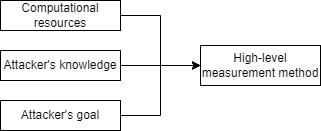
\includegraphics[width=9cm]{pictures/measure_effort.png}
  \caption{Risk indicators of the attacker object in relation to the high-level attributes measurement method.}
  \label{fig:measure_effort}
\end{figure}

\subsection{Using the formal threat model}
\label{sec:use_threat_model}

To measure the extent of damage, subsection \ref{sec:ext_dmg} describe which risk indicators the RMF uses to get the corresponding values. As already explained in subsection \ref{sec:ext_dmg}, these values must be collected from the measurement method of the low-level attributes which explains this subsection how this works. After that, subsection \ref{sec:find_effort} explains how to get the corresponding values for the attacker's effort. The concept to measure the corresponding values that are assigned to the risk indicators describe subsection \ref{sec:find_effort} and is further
explained here by the threat model. In this subsection the research questions \ref{itm:rq2} and \ref{itm:rq3} are addressed in more detail. In reference to the research question \ref{itm:rq4} this
threat model is a possible method for the RMF to measure risks which will be proved in section \ref{sec:evaluation}. As in section \ref{sec:threat} explained, the high- and low-level attributes have to be mapped which this subsection also explains. \\
Before explaining the procedure there are two requirements for the dataset that is collected from the attributes \cite{DBLP:conf/crisis/DoynikovaNGK20} for the analysis process. These requirements are already transferred to ML models:

\begin{enumerate}
  \item The first requirement is a dataset which contains information about the attack actions against a ML model. The information must be based on the skills, resources, intention, and motivation of the attacker.
  \item The second requirment for the dataset is that everything is marked in such a way that the analysis shows which actions the attacker performed. But this requirement is more about having multiple attackers or the analysis accross multiple attackers.
\end{enumerate}

The second requirement can not be fulfilled because this thesis do not differentiate between one or multiple attacker. It is only ever one attacker.

\subsubsection*{The low-level attributes}

To find the extent of damage there is a need to collect data which can be measured from every attack on a ML model. These data are classified and explained in section \ref{sec:threat}. Doynikova et al. \cite{DBLP:conf/crisis/DoynikovaNGK20} explain which data are required to meausre the low-level attributes. The low-level attributes that Doynikova et al. use in their work are event logs, network traffic, namely, and their source that are possible to use in relation with the risk indicators. A possibilty for this is monitoring the values for the risk indicators with event logs, namely, and their source. The network traffic can not be used because the RMF only measures an attack on a ML model locally what does not include MLaaS \cite{DBLP:conf/hci/HaraA21}. \\
The low-level attributes measure the extent of damage based on the collected data. It is therefore important that data about the ML model and the attack can be collected during the entire training and testing process. For example, if the attack specificity needs to be measured then it must be possible to get this through the attack itself. After the assignment of the values Doynikova et al. explain that the low-level attributes must be mapped to the high-level attributes to measure the attacker's effort. The high-level attributes have delimited attributes which are not measured at the low-level attributes. This means the attributes must be evaluated in a separate measurement method afterwards.

\subsubsection*{The high-level attributes}

The high-level attributes measure the values for the attacker's effort based on the risk indicators attacker's knowledge, attacker's goal, and the computational resources. The four groups explained in subsection \ref{sec:threat} are placed in relation to the risk indicators. The first group includes characteristics such as skills, motivation and intention. The motivation and intention correspond to the attacker's goal. The skills are a characteristic that are represented in the knowledge and goal. The second group characterizes the attacker's capabilities \cite{DBLP:journals/iet-cdt/XueGLYO20} and show the characteristics as used resources. This group represents the computational resources. This risk indicators measures which hardware an attacker needs to execute an attack. The third group incorporates the attacker in relation with the attacked system. This group includes the attacker's location, the privileges, his goals, the access and the attacker's knowledge. This part can be used for the RMF with the attacker's goals and knowledge. The attacker's location and privileges are not part of the risk measurement. The last group relates the attacker with the attack and the steps that are included to execute the attack. This group can be used to map the low- and high-level attributes which is explained next.

\subsubsection*{Mapping the low-level with the high-level attributes}
\label{sec:map_low_high}

After explaining the low- and high-level attributes as separated measurement methods, the low- and high-level attributes must be mapped based on the threat model of Doynikova et al. \cite{DBLP:conf/crisis/DoynikovaNGK20}. At this point, the attacks are displayed on the basis of their values. At the beginning, the data of the attacks are measured separately in the measurement method of the low-level attributes and then those of the high-level attributes. The data here always refer to the risk indicators before and after an attack to monitor the original and the manipulated training dataset. Starting with the measurement of the low-level attributes the accuracy and TP, TN, FP, and FN. These risk indicators can be only used to find the extent of damage. The attack time and specificity is relevant for the extent of damage and to find the attacker's effort. This risk indicator gets values that can be transferred to the risk indicators attacker's knowledge and goal. The computational resources are a risk indicator that is only for finding the attacker's effort. Figure \ref{fig:attribute_mapping} summarize this mapping and and in comparison to the threat model of Doynikova et al., the values are completely collected and evaluated without human judgment.

\begin{figure}[ht!]
  \centering
  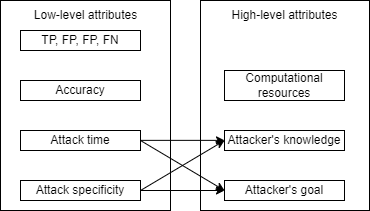
\includegraphics[width=10cm]{pictures/attribute_mapping.png}
  \caption{Mapping between the low- and high-level attributes.}
  \label{fig:attribute_mapping}
\end{figure}

\subsection{Define measurement functions to calculate derived measures}
\label{sec:derived_measures}

In this subsection the base measures are also called risk indicators because the RMF shows the output of the measurement methods assigned to the respective risk indicator. Not every derived measure need to be calculated such as the accuracy and computational resources. The TP, TN, FP, and FN are a risk indicator that can be calculated in a measurement function to different ML metrics such as the accuracy \cite{9783960101925}, confusion matrix \cite{DBLP:journals/isci/XuZM20}, precision-recall \cite{DBLP:conf/icml/DavisG06}, and F1-Score
\cite{9783960101925} which subsection \ref{sec:ml_metrics} describe. This metrics are used to show the differences between an original and poisoned ML model. The derived measures that represent values of the ML model are only calculated from one risk indicator because this risk indicator have multiple different values that are needed to calculate the ML metrics. \\
The risk indicators which are combined to derived measures shows Figure \ref{fig:measurement_steps}. The first derived measure resulting from all values that describe the attack and how and where to execute it. If all of them are combined, then should the derived measure be a value that represents without the computational resources how high the effort is to implement, test, and execute an attack. \\
The combination starts by the attack time and specificity where the attack is executed during training or testing time. If the attack is, for example, executed during testing time, then the concentration is located on all steps after the training of the ML model. If the attack specificity is, for example, untargeted then the attacker can poison the training dataset without finding out label names and only have to add a backdoor trigger. When the attacker decide to implement a backdoor attack then he have to go through pre-determined steps which are defined depending on the used attack. The same applies to the goal which bases on pre-determined steps too. With these information is it possible to combine them and then getting the derived measure. The same procedure combine the measurement function for the extent of damage from the attack time and specificity. The accuracy and computational resources are not considered further here because they are transferred directly to the analytical model.

\begin{figure}[ht!]
  \centering
  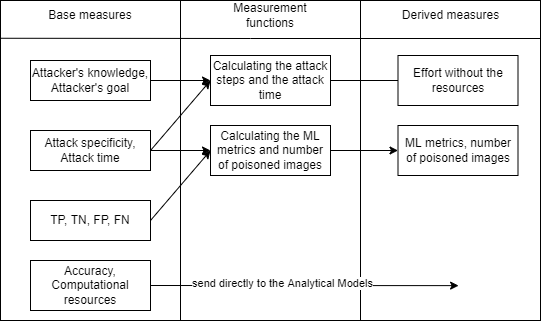
\includegraphics[width=11cm]{pictures/derived_measures.png}
  \caption{Combine the risk indicators to derived measure and evaluate the derived and base measures with the analytical models to indicators.}
  \label{fig:measurement_steps}
\end{figure}

\subsection{Define analytical models and indicators}

The indicators are the final results from the measurement and provide the transition over the decision criteria to the measurement results. After evaluating the derived measures, all measures have to be combined for calculating all values to get the extent of damage and attacker's effort. To get both values, the RMF need to combine the base and derived measures depending on the target value which Figure \ref{fig:indicators} shows. So, the result is, that for this thesis the RMF needs two indicators. Depending on that requirement there have to be two analytical models \cite{ISO_27004_2009}. The analytical models get at this point the function to calculate the measures for the interpretation in the decision criteria. This differentiate from the requirements of analytical models of ISO 27004 \cite{ISO_27004_2009} but is necessary for the risk result which subsection \ref{sec:measurement_results} explains.

\begin{figure}[ht!]
  \centering
  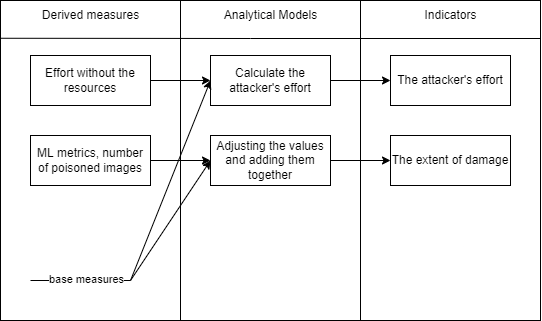
\includegraphics[width=11cm]{pictures/indicators.png}
  \caption{Calculation of the derived and base measures in the analytical models to get the indicators.}
  \label{fig:indicators}
\end{figure}

\subsubsection*{The transition between measurement and measurement results}

After defining the indicators the next step is the transition to the measurement results by interpreting the indicators based on decision criteria. At this position it is important to relate the attacker's effort with the probability of occurrence because this values is used to get the final risk value. \\
The goal for the decision criteria is to interpret the indicators without human judgment. Based on this, the functionality of the decision criteria should decide on given intervals how the indicators can be interpreted. This should make it possible to find the main factor by human judgment that increases the risk value.

\begin{figure}[ht!]
  \centering
  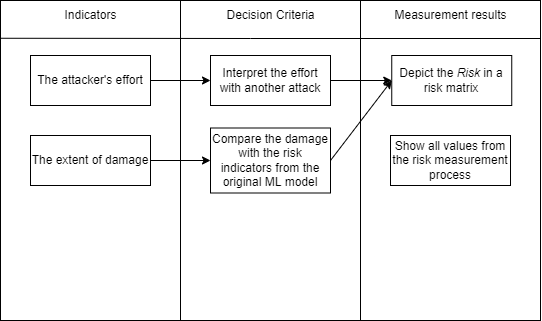
\includegraphics[width=11cm]{pictures/measurement_results_concept.png}
  \caption{Interpreted results that should contain requirements which specify the decision criteria.}
  \label{fig:measurement_results_concept}
\end{figure}

\subsection{Develop measurement results by evaluating the risk measurement}
\label{sec:measurement_results}

The implementation of the measurement results are possible through the decision criteria which are also defined in \cite{ISO_27004_2009}. The RMF show the results as visualized Python plots and calculated results. Both is further explained in section \ref{sec:implementation}.

\subsubsection*{Machine learning metrics for risk measurement}

With regard to poisoning attacks, the goal is to decrease the accuracy \cite{DBLP:conf/icml/BiggioNL12}, \cite{DBLP:journals/corr/abs-1708-06733}. But the RMF should also use the precision-recall, and the F1-score of the training process to show the differences of the training with the original and poisoned training dataset. That should make it possible to identify everything of the attacks. Also with regard to the attacker's effort could be every collected information of the ML model and the training data a possible value.

\subsubsection*{Calculate the risks}

The main calculation is $Risk = $ \textit{Extent of damage} $*$ \textit{Probability of occurrence} \cite{DBLP:journals/access/JianxingHSH21}. This calculation is intended to show how high the risk is for an ML model. Other calculations are displayed in detail as probabilities and stand in relation to the extent of damage or probability of occurance. For example, the composition of the extent of damage from the various risk indicators can be presented again in detail. \\
Now it must be clarified how the probability of occurrence and the extent of damage are represented as values. The probability of occurrence bases on the attacker's effort. This thesis assumes that the higher the effort, the lower the probability of occurrence. The value is represented by a non-negative natural number $x \in \mathbb{N}$ \cite{Morazan2022}. This depends on the number of steps an attacker must perform to execute the attack. The extent of damage is calculated by the addition of all measures. It is important to note that the risk indicators are measured from the differences between the original ML model and the attacked ML model. This combination allows the calculation of a total extent of damage from all individual measures. \\
This risk calculation is classified in a matrix for the extent of damage, a matrix for the attacker's effort, and a matrix that summarizes these matrices by classifying the calculated risk. Figure \ref{fig:sample_matrix} shows a sample matrix where green is the lowest risk level and red the highest. The \textit{x-axis} and \textit{y-axis} show different combinations to classify the values that classify the risk value into the risk matrix.

\begin{figure}[ht!]
  \centering
  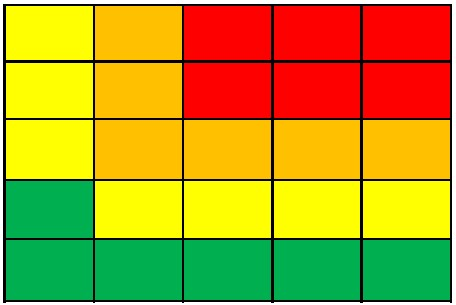
\includegraphics[width=8cm]{pictures/sample_matrix.jpg}
  \caption{Sample risk matrix adapted from \cite{Ivanenko2020IMPLEMENTATIONOR}.}
  \label{fig:sample_matrix}
\end{figure}

This classification bases on the European Telecommunication Standards Institute (ETSI). In their standard \cite{applications_2022}, ETSI show a risk classification standard which table \ref{tab:risk_classify} shows.

\begin{table}[h]
\centering
  \begin{tabular}{|c|p{10cm}|}
  \hline
  \rowcolor{lightgray} Risk & Explanation \\
  \hline
  Minor & ''No essential assets are concerned, or the attack is unlikely. Threats causing minor risks have no
primary need for counter measures.''  \\
  \hline
  Major & ''Threats on relevant assets are likely to occur although their impact is unlikely to be fatal. Major
risks should be handled seriously and should be minimized by the appropriate use of
countermeasures.'' \\
  \hline
  Critical & ''The primary interests of the providers and/or subscribers are threatened and the effort required
from a potential attacker's to implement the threat(s) is not high. Critical risks should be
minimized with highest priority.'' \\
  \hline
  \end{tabular}
\caption{Risk classification adapted from \cite{applications_2022}}
\label{tab:risk_classify}
\end{table}

\subsection{The implementation plan of the RMF}
\label{sec:final_design}

The last point \ref{itm:g} - ''Establishing measurement implementation approach and documentation'' of \ref{sec:standard} shows the needed information for an implementation plan. This subsection shows the final concept as a complete structure. At first a classifier check the trustworthiness of the training data by comparing the training data with trusted training data. To measure the extent of damage there need of an implementation of the low-level attributes. To get the attacker's effort another measurement method should represent the measurement of the high-level attributes. These two classes need to be mapped.

\subsubsection*{The final concept and design for the RMF}

After explaining the expected results the last part of this section shows the summarized concept and design to implement the RMF in the following section. Table \ref{tab:attack} and \ref{tab:attacker} show the two objects with its attributes that represent the risk indicators for the measurement methods afterwards.

\begin{table}[h]
\centering
  \begin{tabular}{|c|p{10cm}|}
  \hline
  \multicolumn{2}{|c|}{Attack object} \\
  \hline
  \rowcolor{lightgray} Attributes & Description \\ [0.5ex]
  \hline
  Accuracy & The accuracy relates the number of data examples with true predicted labels to the number of all examined data examples \cite{9783960101925} \\
  \hline
  TP, FP, TN, FN & This risk indicator can be used to calculate different ML metrics and show its values during the training time \\
  \hline
  Attack specificity & The attack specificity can be targeted or untargeted \\
  \hline
  Attack time & The attack time differentiate between training and deployment time \\
  \hline
  \end{tabular}
\caption{ISO 27004 Object (attack)}
\label{tab:attack}
\end{table}

\begin{table}[h]
\centering
  \begin{tabular}{| c | p{10cm} |}
  \hline
  \multicolumn{2}{|c|}{Attacker object} \\
  \hline
  \rowcolor{lightgray} Attributes & Description \\ [0.5ex]
  \hline
  Attacker's goal & The attacker's goal can be a denial-of-service, doing an inference failure, or obtaining secret information \\
  \hline
  Attacker's knowledge & The knowledge of an attacker can be categoraized between white-, black-, or grey-box \\
  \hline
  Computational resources & The CPU, memory, GPU are the three parts which represent the used effort from the computer to attack and train a ML model. \\
  \hline
  \end{tabular}
\caption{ISO 27004 Object (attacker)}
\label{tab:attacker}
\end{table}

In Figure \ref{fig:complete_architecture} the identified risk indicators are passed to the measurement methods which are one of the two main components for the risk measurement. As next must the backdoor attacks selected to measure the value that are assigned for the next main component, the measurement which follows the requirements from ISO 27004 \cite{ISO_27004_2009}.

\begin{figure}[ht!]
  \centering
  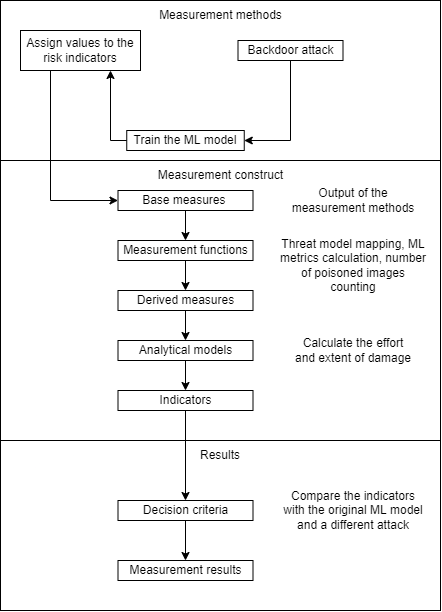
\includegraphics[width=8cm]{pictures/complete_architecture.png}
  \caption{Complete concept architecture adapted from \cite{ISO_27004_2009}.}
  \label{fig:complete_architecture}
\end{figure}

\subsection{Expected results of the RMF}

After attacking a ML model without considering the defense, the values of the accuracy of the poisoned data should be lowest value (\%) as possible which is the highest effectiveness of the attack. The accuracy of the original training and testing should be completely unchanged or so minimally changed that it is not noticeable. The attack time should always recognize that the attack is executed during training time because all attacks in this thesis are backdoor attacks. Attack specificity should be always find if an attack is targeted or untargeted if the attacker whether the attacker specifies a target or not. Attacker's goal should reproduce the steps of an attacker based on the attack to find the goal of that attack. Attacker's knowledge should measure the attacks depending if it is a white- or black-box attack, which attack time, and attack specificity is measured before. The risk result of the risk measurement without any defenses of the ML model should be the worst possible risk level in the risk matrix. In conclusion, however, it is not possible to expect that the evaluation of the risk measurement can say how high or low the risk is.
